\documentclass[11pt,letterpaper]{article}
\usepackage[margin=1in,headheight=15pt]{geometry}
\usepackage[T1]{fontenc}
\usepackage{newtxtext}
\usepackage{mathtools,amsthm}
\usepackage{newtxmath}
\usepackage{microtype}
\usepackage{booktabs,array,longtable,enumitem}
\usepackage[dvipsnames]{xcolor}
\usepackage{tikz}
\usepackage[most]{tcolorbox}
\usepackage{fancyhdr}
\usepackage{xurl}
\usepackage{hyperref}
\definecolor{ink}{HTML}{18364A}
\definecolor{accent}{HTML}{147D92}
\definecolor{pale}{HTML}{EFF6F8}
\hypersetup{colorlinks=true,linkcolor=ink,citecolor=accent,urlcolor=accent,
  pdftitle={Unique Histories from Linear Equations},
  pdfauthor={Research report prepared for Vladimir Reshetnikov},
  pdfsubject={Canonical cellular computation over the polynomial semiring N[X,Y]}}
\pagestyle{fancy}
\fancyhf{}
\fancyhead[L]{\small\scshape Unique Histories from Linear Equations}
\fancyhead[R]{\small ProveIt research report}
\fancyfoot[C]{\thepage}
\renewcommand{\headrulewidth}{0.3pt}
\setlength{\parskip}{4pt}
\setlength{\parindent}{1.2em}
\setlist{itemsep=3pt,topsep=5pt}
\setcounter{tocdepth}{2}
\numberwithin{equation}{section}
\newtheorem{theorem}{Theorem}[section]
\newtheorem{lemma}[theorem]{Lemma}
\newtheorem{proposition}[theorem]{Proposition}
\newtheorem{corollary}[theorem]{Corollary}
\theoremstyle{definition}
\newtheorem{definition}[theorem]{Definition}
\newtheorem{remark}[theorem]{Remark}
\newcommand{\N}{\mathbb N}
\newcommand{\Z}{\mathbb Z}
\newcommand{\Qfield}{\mathbb Q}
\newcommand{\Sring}{\mathcal S}
\newcommand{\A}{\mathcal A}
\newcommand{\F}{\mathcal F}
\newcommand{\supp}{\operatorname{supp}}
\newcommand{\wt}{\operatorname{wt}}
\newcommand{\rep}[1]{[#1]_X}
\newcommand{\LL}{\mathsf L}
\newcommand{\CC}{\mathsf C}
\newcommand{\RR}{\mathsf R}
\newcommand{\OO}{\mathsf O}
\newcommand{\epsa}{\delta_{a,0}}
\newcommand{\System}{\ensuremath{\mathcal E_{f,\F}(w)}}
\newcommand{\repo}{\texttt{ProveIt}}
\newtcolorbox{statementbox}{colback=pale,colframe=accent,boxrule=0.6pt,
  arc=1pt,left=9pt,right=9pt,top=7pt,bottom=7pt,breakable}
\newcommand{\codename}[1]{\texttt{\small #1}}

\begin{document}
\begin{titlepage}
\thispagestyle{empty}
\vspace*{0.5in}
{\color{accent}\large\scshape Computability \; / \; Polynomial semirings}\par
\vspace{0.3in}
{\color{ink}\fontsize{29}{34}\selectfont\bfseries
Unique Histories\par from Linear Equations\par}
\vspace{0.24in}
{\Large A canonical cellular-computability compiler\par
 over $\N[X,Y]$}\par
\vspace{0.35in}
{\large Research report prepared for Vladimir Reshetnikov}\par
{\large 2 October 2026}\par
\vspace{0.35in}
\begin{abstract}
We give a complete affine-linear encoding of finite cellular computations in
polynomials with nonnegative integer coefficients. For a deterministic
radius-one cellular automaton with $s$ symbols, a quiescent blank, and a
designated accepting alphabet, the compiler has exactly $s^3+s+5$ polynomial
unknowns. The direct symbol-marginal form uses $3s+3$ equations; an exact
binary-feature reduction uses $3\lceil\log_2s\rceil+6$ equations with unit
coefficients. Allowing coefficients of magnitude at most $s-1$ gives just
nine equations for $s\ge2$. Every matrix is independent of the input word
and running time; its entries have at most two monomials and coordinate
total degree at most three.

The solution set is empty unless the first accepting configuration has
exactly one accepting cell. In that case the entire polynomial witness is
unique, and all its coefficients are zero or one. Conservation equations
force a canonical expanding space--time region, so neither occupancy
inequalities nor an externally chosen time horizon is needed. A marginal
projection removes $(s-1)^2$ equations from a pair-colour compiler without
changing any natural-polynomial solution tuple. Injective symbol features
compress the same witnesses further without introducing new variables.

We prove $\Sigma^0_1$-completeness for a fixed matrix, an exact
running-time/degree correspondence, a noncomputable degree-bound theorem,
a parsimonious nondeterministic extension, and a single quadratic equation
with the same solutions. We also give an executable compiler, exhaustive
finite checks, and a fully expanded worked quadratic. The contribution is
an explicit uniqueness-preserving normal form, not the already known
undecidability of linear polynomial-semiring equations, and not an ordinary
single-fold Diophantine representation over the natural numbers.
\end{abstract}
\vfill
\begin{statementbox}
\textbf{Status.} Complete mathematical arguments and reproducible exact
computations are supplied. This is an unrefereed research manuscript, not a
Lean or Rocq formalization. Historical priority for the particular combined
normal form has not been established. The distinction between polynomial
unknowns and ordinary integer unknowns is essential throughout.
\end{statementbox}
\end{titlepage}

\tableofcontents
\newpage

\section{The question and the result}
\label{sec:intro}

A finite computation can be certified by introducing variables for each
successive state. The number of variables then grows with the chosen time
horizon. A different question is whether an entire, arbitrarily long
computation can be represented by a fixed number of algebraic objects while
retaining a precise correspondence between computations and complete
witnesses. Here the algebraic objects are finite polynomials: the number of
unknown polynomials stays fixed, whereas their degrees and supports grow
with the computation.

The main technical issue is not merely to encode local transition rules.
It is to prevent additional tiles, detached components, multiplicities,
extra blank padding, independently chosen clock lengths, and arbitrary
accepting continuations from creating spurious or duplicate witnesses.
The construction below resolves these issues within a particularly simple
syntax: affine-linear equations over the semiring $\N[X,Y]$.

\subsection{Main normal-form theorem}

Throughout, $\N=\{0,1,2,\ldots\}$. An accepting event means that at least one
cell carries a symbol from a designated set $\F$. A \emph{first singleton
acceptance} is a first accepting event at which exactly one cell is
accepting. This condition is automatic for the usual one-head simulation
of a deterministic accepting Turing machine, but is not automatic for an
arbitrary cellular automaton.

\begin{theorem}[Canonical linear history compiler]
\label{thm:main}
Let $\A$ be a finite alphabet of size $s$, with blank symbol $0$. Let
$f:\A^3\to\A$ satisfy $f(0,0,0)=0$, and let
$\F\subseteq\A\setminus\{0\}$. There is an explicitly constructible matrix
\[
  \mathsf A_{f,\F}\in
  \Z[X,Y]^{(3s+3)\times(s^3+s+5)}
\]
and an effective encoding of each nonempty finite word $w$ as a vector
$\mathsf b(w)$ of zero--one coefficient polynomials such that:
\begin{enumerate}[label=\textup{(\roman*)}]
\item $\mathsf A_{f,\F}U=\mathsf b(w)$ has a solution
      $U\in\N[X,Y]^{s^3+s+5}$ precisely when the evolution from $w$, with
      blank exterior, has a first singleton acceptance.
\item Whenever a solution exists, the complete tuple $U$ is unique and
      every coefficient in every component of $U$ is zero or one.
\item If the first acceptance time is $h$ and the input length is $m$, then
\[
 \max_i\deg_Y U_i=h,\qquad
 \max_i\deg_X U_i=m+2h+1,\qquad
 \max_i\deg U_i=m+3h+1.
\]
\item Every nonzero matrix entry has at most two monomials, with
      coefficients in $\{-1,1\}$ and total degree at most three.
      The matrix depends only on $f$ and $\F$, not on $w$, $m$, or $h$.
\end{enumerate}
\end{theorem}

The theorem is proved in Sections~\ref{sec:compiler}--\ref{sec:correctness}.
It is a statement about all solutions, not only about a specially
constructed class of well-behaved solutions. No coefficient bounds,
monomial predicates, support bounds, or time indices are added as hidden
side conditions.

\begin{corollary}[A fixed unambiguous hard instance family]
\label{cor:hard-intro}
For one fixed choice of $f$ and $\F$, deciding whether
$\mathsf A_{f,\F}U=\mathsf b(w)$ is solvable over $\N[X,Y]$ is
$\Sigma^0_1$-complete. Every input word in this family has either no solution
or exactly one solution, and any solution has only zero--one coefficients.
\end{corollary}

The direct form of Theorem~\ref{thm:main} is convenient for understanding
soundness. Section~\ref{sec:features} proves two stronger row counts with
\emph{exactly the same complete solution tuples}: $3\lceil\log_2s\rceil+6$
rows retaining unit coefficients, or nine rows allowing coefficients of
magnitude at most $s-1$ for $s\ge2$. All conclusions about uniqueness,
Boolean coefficients, and degrees transfer unchanged.

The proof uses a direct one-head Turing-machine simulation, not an
assumption that an arbitrary cellular rule is universal. The construction
of that simulation is given in Section~\ref{sec:universality}.

\subsection{What is and is not new here}

Narendran proved undecidability of systems of linear equations over
polynomial semirings, already with one indeterminate, in 1996
\cite{Narendran}. Thus neither polynomial-semiring undecidability nor
monomial forcing is claimed as a new idea. In particular, the elementary
power-forcing equations used below have a predecessor in his construction.

Lohrey and Steinberg encode Turing machines by tilings to obtain
undecidable subsemimodule membership for finite-rank free
$(\Z\times\Z)$-modules, and related group-theoretic results
\cite{LohreySteinberg}. Their zero-tiling-sum formulation permits multiple
tiles at a location. It is a close conceptual precedent for interpreting
linear equations as translated local constraints.

The contribution developed here is the combined, explicitly counted
normal form: a fixed low-degree matrix, exact shape recovery from
conservation, first-acceptance canonicalization, uniqueness of every
auxiliary polynomial, forced zero--one coefficients, and an exact degree
ledger. These properties are proved directly. We have not established that
this precise combination is absent from all earlier literature, and do
not present the theorem as a resolution of a named longstanding
Diophantine conjecture.

Dong's work provides a useful contrast: a single homogeneous linear
equation over $\N[X]$ admits polynomial-time decision procedures for the
nonzero-solution problem he studies \cite{Dong}. This is not a decision
procedure for arbitrary inhomogeneous systems. The contrast here is
therefore not a claimed one-variable/two-variable undecidability threshold.
Two coordinate indeterminates are used because they retain the actual
space--time geometry transparently.

\subsection{Connection with the repository}

The inspected \repo{} snapshot contains both formalized MRDP material and
many computational-substrate certificate projects. Its Hilbert-tenth
README carefully distinguishes finite-horizon compilers from fixed
universal arithmetic bounds and records a 75-operation certificate /
87-operation universal-polynomial boundary for a separate natural-number
construction \cite{ProveIt}. This report changes neither of those counts.

Instead, it contributes a different target domain and a potentially useful
intermediate representation. The polynomial tuple is canonical before
any attempt is made to pack it into ordinary integers. The transferable
parts are the proof of shape, the marginal and feature projections, the witness
reconstruction theorem, and the explicit conditions that a later packing
stage must preserve. No repository theorem is used as an unexamined
black-box lemma in the elementary compiler proof.

\section{Semantics and notation}
\label{sec:semantics}

\subsection{Polynomials are the unknown values}

Let
\[
  \Sring=\N[X,Y]\subset\Z[X,Y].
\]
An element of $\Sring$ is a finite sum
$P=\sum_{i,j\ge0}p_{ij}X^iY^j$ with $p_{ij}\in\N$.
The symbols $X,Y$ are fixed coordinate indeterminates, not existentially
quantified numbers. An equation is an identity of polynomials, equivalent
to equality at every coefficient.

A linear system means
\begin{equation}
  \sum_{j=1}^n a_{ij}(X,Y)U_j(X,Y)=b_i(X,Y),
  \qquad 1\le i\le r,
  \label{eq:linear-semantics}
\end{equation}
where the $a_{ij},b_i$ are supplied integer-coefficient polynomials and
$U_j\in\Sring$ are unknown. There are no products $U_jU_k$ in a linear
system. Negative coefficient terms in~\eqref{eq:linear-semantics} may be
moved to the opposite side, so this is equally an equality between two
expressions formed with addition and multiplication by fixed elements
of $\Sring$.

We call a representation \emph{single-fold over $\Sring$} when every
admitted input has exactly one full tuple of $\Sring$-witnesses, and every
other input has none. This terminology does not change the domain to
$\N$. One polynomial variable contains an unbounded finite amount of data.

Write
\[
 \rep{r}=1+X+\cdots+X^{r-1},\qquad \rep{0}=0.
\]
For a nonnegative polynomial, its mass is
$\wt(P)=P(1,1)$, the sum of all coefficients. A polynomial is called
\emph{Boolean-coefficient} when all its coefficients belong to
$\{0,1\}$; no Boolean-ring arithmetic is intended. We use $\deg 0=-\infty$ for total
and coordinate degrees, so maxima over tuples with zero components are
unambiguous.

\subsection{The cellular evolution}

Let $w=w_0\cdots w_{m-1}\in\A^m$, $m\ge1$. The initial configuration is
\[
 c_0(i)=\begin{cases}w_i,&0\le i<m,\\0,&\text{otherwise},\end{cases}
 \qquad i\in\Z.
\]
Subsequent configurations satisfy
\begin{equation}
 c_{t+1}(i)=f(c_t(i-1),c_t(i),c_t(i+1)).
 \label{eq:ca}
\end{equation}
Quiescence gives the elementary light-cone bound
\begin{equation}
 c_t(i)=0\quad\text{if }i<-t\text{ or }i>m-1+t.
 \label{eq:cone}
\end{equation}
Indeed, a cell outside the larger interval at time $t+1$ has three blank
predecessors at time $t$. This proves~\eqref{eq:cone} by induction.

We distinguish \emph{configuration rows} from \emph{transition rows}.
Transition row $t$ contains the triples whose centres are
\[
 i=-t-1,-t,\ldots,m+t.
\]
There are
\begin{equation}
 w_t=m+2t+2
 \label{eq:width}
\end{equation}
such triples. The two extreme centres are blank guard cells at time $t$;
their outputs are allowed to become nonblank at time $t+1$. We encode the
centre $i$ in this row at horizontal exponent
\begin{equation}
  j=i+t+1,\qquad 0\le j<w_t.
  \label{eq:shear}
\end{equation}
Thus a cell remaining at physical position $i$ shifts one place to the
right when moving to the next encoded row. This is the source of the
factor $XY$ in the vertical equations.

\section{A finite nonnegative flow forces a clock}
\label{sec:clocks}

The following elementary lemma is the main mechanism for obtaining exact
shape information from linear equations. Its power-forcing special cases
are familiar from polynomial-semiring undecidability constructions
\cite{Narendran}; the translated form is convenient for the present proof.

\begin{lemma}[Ray-clock lemma]
\label{lem:ray}
Let $S=X^aY^b$ and $M=X^pY^q$, where $a,b,p,q\in\N$ and $p+q>0$.
For $U,V\in\Sring$, the identity
\begin{equation}
 U+V=S+MV
 \label{eq:ray}
\end{equation}
holds if and only if, for some $h\in\N$,
\begin{equation}
 U=SM^h,\qquad V=S\sum_{t=0}^{h-1}M^t.
 \label{eq:ray-sol}
\end{equation}
The integer $h$ is uniquely determined, and equals $\wt(V)$.
\end{lemma}

\begin{proof}
Evaluation at $(1,1)$ gives $\wt(U)=1$. Hence $U$ is a monomial with
coefficient one. Regard the coefficients of $V$ as nonnegative integer
flows along directed edges
\[
 (i,j)\longrightarrow(i+p,j+q)
\]
in $\N^2$. Equation~\eqref{eq:ray} says that the unique source is at
$(a,b)$ and the unique sink is at the exponent of $U$. Every vertex has at
most one predecessor and one successor, and total degree strictly
increases along every edge.

For completeness, this flow description can be checked purely by
coefficient induction. Before the source, and on every chain not meeting
the source, the incoming coefficient is zero. A positive outgoing
coefficient cannot appear there without a source; a sink there would
force a negative coefficient. At the source the outgoing coefficient is
one unless the sink is the source itself. That coefficient remains one
along its unique successor chain until the sink is reached. Since $V$
has finite support, this chain must terminate at the sink. There can be
no other flow. It follows that the sink is $SM^h$ and that precisely the
first $h$ edges of this ray carry coefficient one. This is
\eqref{eq:ray-sol}. Conversely, those expressions satisfy
\eqref{eq:ray} by telescoping. Their mass and uniqueness statements follow
immediately.
\end{proof}

Two aspects matter. First, finiteness of support excludes an infinite
unterminated flow. Second, nonnegativity excludes a compensating signed
flow on another chain. Ordinary scalar evaluation of the equation does
not retain either of these coefficientwise arguments.

\section{The complete compiler}
\label{sec:compiler}

We now list every unknown and every equation. The list itself is the
compiler; no separate validity predicate is attached to its output.

\subsection{Unknown polynomials and linear forms}

For each triple $\tau=(\ell,c,r)\in\A^3$, introduce a polynomial
$Z_{\ell c r}$. Its intended coefficient at $X^jY^t$ is one when that
triple occurs at transition site $(j,t)$, and zero otherwise. Introduce
$T_a$ for every $a\in\A$ to record the final configuration, with one blank
guard at either end. Introduce five further polynomials
\[
 D,\ Q,\ B,\ V,\ J.
\]
These are all the unknowns, giving $s^3+s+5$ in total.

For $a\in\A$, use the following abbreviations for \emph{linear forms},
not additional unknowns:
\begin{align}
 \LL_a&=\sum_{\ell=a}Z_{\ell c r}, &
 \CC_a&=\sum_{c=a}Z_{\ell c r},\label{eq:marginals1}\\
 \RR_a&=\sum_{r=a}Z_{\ell c r}, &
 \OO_a&=\sum_{f(\ell,c,r)=a}Z_{\ell c r}.
 \label{eq:marginals2}
\end{align}
Indices not specified under a sum range independently over $\A$.
Also put
\begin{equation}
 I_a(X)=\sum_{\substack{0\le j<m\\ w_j=a}}X^j,
 \qquad G=V+B+Q+D.
 \label{eq:input-ghosts}
\end{equation}
The $I_a$ are supplied data, and $G$ is another linear form.

\subsection{Equations}

The two clocks are
\begin{align}
 D+Q&=X^{m+1}+X^2YQ, \tag{C1}\label{eq:C1}\\
 B+V&=1+YV. \tag{C2}\label{eq:C2}
\end{align}
The left-neighbour marginal equations, one for every $a\in\A$, are
\begin{equation}
 X\CC_a+\epsa V=\LL_a+\epsa XQ.
 \tag{L$_a$}\label{eq:L}
\end{equation}
The right-neighbour marginal equations are needed only for nonblank
symbols:
\begin{equation}
 X\RR_a=\CC_a\qquad (a\in\A\setminus\{0\}).
 \tag{R$_a$}\label{eq:R}
\end{equation}
The vertical equations, one for each symbol, are
\begin{equation}
 \CC_a+T_a=XI_a+XY\OO_a+\epsa G.
 \tag{V$_a$}\label{eq:V}
\end{equation}
Finally, acceptance is enforced by
\begin{align}
 \sum_{a\in\F}\CC_a&=0, \tag{F0}\label{eq:F0}\\
 \sum_{a\in\F}T_a+J&=B+XJ. \tag{F1}\label{eq:F1}
\end{align}
All equalities are polynomial identities, and every listed unknown ranges
over $\Sring$.

\begin{table}[ht]
\centering
\begin{tabular}{@{}llr@{}}
\toprule
Component & Role & Number of rows\\
\midrule
\eqref{eq:C1}--\eqref{eq:C2} & Right boundary and vertical clock & $2$\\
\eqref{eq:L} & Left-neighbour matching and total shape & $s$\\
\eqref{eq:R} & Right-neighbour matching, blank row omitted & $s-1$\\
\eqref{eq:V} & Input, transition, and terminal row & $s$\\
\eqref{eq:F0}--\eqref{eq:F1} & First singleton acceptance & $2$\\
\midrule
Total & Complete affine-linear system & $3s+3$\\
\bottomrule
\end{tabular}
\caption{No occupancy rows or coefficient-Booleanity equations are added.}
\label{tab:rowledger}
\end{table}

\subsection{Why the matrix is fixed}

Move the supplied terms $X^{m+1}$, $1$, and $XI_a$ to the right-hand
vector, leaving every unknown on the left. The remaining coefficient
polynomials depend only on the alphabet, the rule table, and the
accepting set. Typical entries are $1-X^2Y$, $1-Y$, $X-1$, $1-XY$,
$1-X$, $X$, and $-1$. For an individual tile variable there is at most
one positive and one negative occurrence in any row. Thus each entry has
at most two monomials with coefficients of magnitude at most one, and
total coordinate degree at most three.

The apparent input-dependent coefficient in a naive boundary construction
would be $X^{m+1}Q$. It does not occur here. Instead, the right-boundary
clock is \emph{started} at $X^{m+1}$ in the supplied constant term of
\eqref{eq:C1}. All subsequent shifts are multiplication by the fixed
monomial $X^2Y$. This is the step that makes the matrix independent of the
input length.

\section{Shape and soundness}
\label{sec:correctness}

\subsection{The clocks synchronize without a separate equation}

\begin{lemma}[Forced boundary and transition region]
\label{lem:shape}
Every solution of the complete system has a uniquely determined
$h\in\N$ for which
\begin{align}
 D&=X^{m+1+2h}Y^h,
 &Q&=\sum_{t=0}^{h-1}X^{m+1+2t}Y^t,\label{eq:DQ}\\
 B&=Y^h,
 &V&=\sum_{t=0}^{h-1}Y^t.\label{eq:BV}
\end{align}
Moreover, the total tile polynomial $H=\sum_{\ell,c,r}Z_{\ell c r}$ is
\begin{equation}
 H=\sum_{t=0}^{h-1}Y^t\rep{m+2t+2}.
 \label{eq:Hshape}
\end{equation}
Consequently, at every site in this region exactly one tile polynomial
has coefficient one, and all tile coefficients outside the region vanish.
\end{lemma}

\begin{proof}
Apply Lemma~\ref{lem:ray} separately to \eqref{eq:C1} and
\eqref{eq:C2}. This gives~\eqref{eq:DQ} for one integer $h$ and gives
$B=Y^k$, $V=\sum_{t<k}Y^t$ for a possibly different integer $k$.

Summing all equations~\eqref{eq:L} over $a$ uses
$\sum_a\CC_a=\sum_a\LL_a=H$ and yields
\begin{equation}
 XH+V=H+XQ.
 \label{eq:sumL}
\end{equation}
Evaluation at $(1,1)$ gives $k=h$. Thus the two clocks have the same
height without a separately paid synchronization variable or row.

Rearrange~\eqref{eq:sumL}:
\[
 (1-X)H=V-XQ
  =\sum_{t=0}^{h-1}Y^t(1-X^{m+2t+2}).
\]
Since $(1-X)\rep{r}=1-X^r$, the displayed expression for $H$ satisfies
this equation. It is the only such polynomial, because $1-X$ is not a
zero divisor in $\Z[X,Y]$.

Every coefficient of every $Z_{\ell c r}$ is nonnegative. Their sum is
one at each site of~\eqref{eq:Hshape}, and zero elsewhere. Therefore
exactly one tile is present at each permitted site, with coefficient one;
no tile can occur elsewhere or with multiplicity greater than one.
\end{proof}

This argument establishes occupancy rather than assuming it. In
particular, it rules out disjoint extra computations and translated closed
components: their nonnegative coefficients would alter the forced total
$H$.

\subsection{The terminal region is also forced}

\begin{lemma}[Forced top row]
\label{lem:top}
Every solution satisfies
\begin{equation}
 K:=\sum_{a\in\A}T_a=Y^h\rep{m+2h+2}.
 \label{eq:topshape}
\end{equation}
At each site of this row exactly one terminal symbol occurs with
coefficient one; every terminal coefficient elsewhere is zero.
\end{lemma}

\begin{proof}
Each triple has exactly one central symbol and exactly one output under
$f$. Hence $\sum_a\CC_a=\sum_a\OO_a=H$. Also,
$\sum_a I_a=\rep{m}$. Summing~\eqref{eq:V} gives
\begin{equation}
 H+K=X\rep{m}+XYH+G.
 \label{eq:sumV}
\end{equation}
By~\eqref{eq:DQ}--\eqref{eq:BV},
\begin{equation}
 G=\sum_{t=0}^{h}Y^t(1+X^{m+2t+1}).
 \label{eq:Gshape}
\end{equation}
The coefficient row at $Y^0$ on the right of~\eqref{eq:sumV} is
$X\rep{m}+1+X^{m+1}=\rep{m+2}$. For $1\le t\le h$, that row is
\[
 X\rep{m+2t}+1+X^{m+2t+1}=\rep{m+2t+2}.
\]
There are no other rows. Subtracting the already known $H$ leaves exactly
\eqref{eq:topshape}. This argument includes $h=0$, when $H=0$ and the
initial guarded row is already the top row. Nonnegativity now proves the
one-symbol-per-site assertion just as in Lemma~\ref{lem:shape}.
\end{proof}

\subsection{Neighbour matching is exact}

The omitted blank right-neighbour row is not a missing constraint.
Summing~\eqref{eq:R} over $a\ne0$ and subtracting that sum from
\eqref{eq:sumL} gives
\begin{equation}
 X\RR_0+V=\CC_0+XQ.
 \label{eq:Rzero}
\end{equation}
Thus, with the blank boundary terms restored, right-neighbour matching
holds for every symbol.

\begin{lemma}[The tile triples are genuine consecutive windows]
\label{lem:windows}
Fix a transition row $t<h$, and write its unique tile at position $j$ as
$(\ell_j,c_j,r_j)$, for $0\le j<w_t$. Then
\[
 \ell_0=c_0=0,\qquad c_{w_t-1}=r_{w_t-1}=0,
\]
and for $1\le j<w_t$,
\[
 \ell_j=c_{j-1},\qquad c_j=r_{j-1}.
\]
In particular, the tile at each site is the actual length-three window
of the row of centre symbols, with blank exterior.
\end{lemma}

\begin{proof}
At an interior position $j$, coefficient comparison in \eqref{eq:L}
gives the equality of the one-symbol indicators of $c_{j-1}$ and
$\ell_j$. The right-neighbour rows, including~\eqref{eq:Rzero}, give
the equality of the indicators of $r_{j-1}$ and $c_j$. Since the
occupancy lemma has already proved that these are single symbols, the
indicator equalities imply the asserted equalities of symbols.

At position zero, \eqref{eq:L} forces $\ell_0=0$ and the right-neighbour
rows force $c_0=0$. At the coefficient immediately after the last tile,
the boundary monomial in $XQ$ forces $c_{w_t-1}=0$ in the left rows and
$r_{w_t-1}=0$ in the right rows. All boundary exponents agree with
\eqref{eq:width} by~\eqref{eq:DQ}. Finally, the interior equalities also
give $r_j=c_{j+1}$ wherever that expression is internal to the row.
\end{proof}

It would not be sound to deduce equality of joint symbol pairs from
marginal counts before proving occupancy. Here occupancy comes first;
there is exactly one tile, not a distribution or a multiset, at a site.

\subsection{Vertical matching recovers the actual evolution}

\begin{lemma}[Semantic reconstruction]
\label{lem:reconstruct}
For each $t<h$, the coefficient of $X^jY^t$ in $\CC_a$ is one exactly
when
\[
 c_t(j-t-1)=a,\qquad 0\le j<w_t.
\]
The coefficient of $X^jY^h$ in $T_a$ is one exactly when
$c_h(j-h-1)=a$, for $0\le j<w_h$.
\end{lemma}

\begin{proof}
When $h>0$, the $Y^0$ part of~\eqref{eq:V} is
\[
 \CC_a\big|_{Y^0}=XI_a+\epsa(1+X^{m+1}).
\]
This is precisely the input configuration with the two source guards.
By Lemma~\ref{lem:windows}, every tile in this row contains the true
neighbourhood of its centre. Its assigned output is therefore the true
cellular output. Multiplication by $XY$ moves that output to the next
encoded source row and shifts its exponent by one, as required by
\eqref{eq:shear}. The two new boundary terms in $G$ supply the blank
source guards for that row. Inducting in $t$ recovers all transition
rows.

At time $h$, there are no centre terms because $H$ has no $Y^h$ row.
Equation~\eqref{eq:V} therefore places the last outputs, together with
the guards, in the $T_a$. This proves the terminal assertion. If $h=0$,
the same equation directly reads
$T_a=XI_a+\epsa(1+X^{m+1})$, which proves the assertion without a
transition row. Bound~\eqref{eq:cone} and quiescence ensure that the
omitted infinite exterior is genuinely blank, not an unverified part of
the computation.
\end{proof}

\subsection{Acceptance and all auxiliary witnesses}

\begin{lemma}[First acceptance and the horizontal marker]
\label{lem:acceptance}
Every solution encodes a first singleton acceptance at time $h$. If its
accepting cell has encoded horizontal position $j_*$, then
\begin{equation}
 \sum_{a\in\F}T_a=X^{j_*}Y^h,
 \qquad J=Y^h\rep{j_*},
 \qquad 1\le j_*\le m+2h.
 \label{eq:J}
\end{equation}
\end{lemma}

\begin{proof}
All summands in~\eqref{eq:F0} are nonnegative. Thus no centre row before
$h$ has an accepting symbol. Lemma~\ref{lem:reconstruct} identifies
these with the genuine configurations, including their blank exterior.

Apply Lemma~\ref{lem:ray} to~\eqref{eq:F1}, with source $B=Y^h$,
multiplier $X$, and sink $\sum_{a\in\F}T_a$. It yields exactly the first
two formulas in~\eqref{eq:J}. There is consequently one accepting cell
at time $h$, not merely a selected cell among several. The two top
boundary cells are blank by the vertical reconstruction and $0\notin\F$,
which gives the stated bounds on $j_*$. The marker $J$ is uniquely forced;
there is no slack in its choice.
\end{proof}

\subsection{Completeness and uniqueness}

\begin{proof}[Completion of the proof of Theorem~\ref{thm:main}]
Suppose first that the genuine evolution has a first singleton acceptance
at time $h$. Define $D,Q,B,V$ by~\eqref{eq:DQ}--\eqref{eq:BV}. At every
transition site $(j,t)$ with $t<h$, put coefficient one in the unique
$Z_{\ell c r}$ corresponding to the actual neighbourhood of physical
centre $j-t-1$. Put coefficient one in $T_a$ at $(j,h)$ according to the
actual guarded final row. Define $J$ by~\eqref{eq:J}. All unspecified
coefficients are zero.

The clock equations telescope. The spatial equations express exact
adjacency and the blank source boundaries. The vertical equations express
the input row, the deterministic rule, and the two new guards at each
stage. The absence of earlier acceptance gives~\eqref{eq:F0}, and the
single terminal accepting cell gives~\eqref{eq:F1}. Thus this tuple is a
solution, proving completeness.

Conversely, the preceding lemmas reconstruct a genuine first singleton
acceptance from every solution. The first accepting time of a
deterministic evolution is unique. Hence every solution must have the
same $h$. Its clocks are then fixed, every transition tile and terminal
symbol is fixed by the actual evolution, and $J$ is fixed by the location
of the accepting cell. There is therefore exactly one full solution
tuple. All its components are Boolean-coefficient by the construction and
by the shape and clock lemmas. The matrix-size and coefficient assertions
were checked in Section~\ref{sec:compiler}; the exact degree assertions
are proved in Section~\ref{sec:resources} below.
\end{proof}

\begin{remark}[Two accepting cells are not one accepting certificate]
If the first accepting configuration contains two or more accepting
cells, the system has no solution. A later time with only one accepting
cell cannot help, because \eqref{eq:F0} detects the earlier event. For
arbitrary cellular automata this restriction is part of the specified
language, not an omitted case in the theorem. One-head machine encodings
satisfy it automatically.
\end{remark}

\section{An exact marginal projection}
\label{sec:projection}

A more direct tile formulation would use the ordered pair of symbols on
each side of a tile as its horizontal colour. Define
\[
 W_{ab}=\sum_{(\ell,c)=(a,b)}Z_{\ell c r},\qquad
 E_{ab}=\sum_{(c,r)=(a,b)}Z_{\ell c r}.
\]
The pair-colour spatial equations are
\begin{equation}
 XE_{ab}+\delta_{a,0}\delta_{b,0}V
   =W_{ab}+\delta_{a,0}\delta_{b,0}XQ,
 \qquad a,b\in\A.
 \label{eq:pair}
\end{equation}
Together with the same clocks, vertical equations, and acceptance rows,
these give $s^2+s+4$ equations on exactly the same witness tuple.

\begin{theorem}[Full-tuple preservation under marginal reduction]
\label{thm:projection}
The pair-colour system and the reduced system \System{} have identical
solution sets in $\Sring^{s^3+s+5}$. Replacing~\eqref{eq:pair} by
\eqref{eq:L}--\eqref{eq:R} removes exactly $(s-1)^2$ equations and changes
neither the meaning nor the value of any witness coordinate.
\end{theorem}

\begin{proof}
Sum~\eqref{eq:pair} over $b$ for fixed $a$. The resulting equation is
\eqref{eq:L}. Sum it over $a$ for fixed $b$ to obtain the complete
right-neighbour equation for $b$; discarding its blank instance gives
\eqref{eq:R}. Thus every pair-colour solution is a reduced solution.

For the reverse implication, Lemma~\ref{lem:shape} proves that each site
contains one tile, and Lemma~\ref{lem:windows} proves equality of both
components of the adjacent pair. Therefore the ordered pairs themselves
agree. At the left and right boundaries the pair is $(0,0)$, and there
are no tiles outside the prescribed region. Comparing coefficients at
every site gives~\eqref{eq:pair}. The equation-count difference is
\[
 (s^2+s+4)-(3s+3)=(s-1)^2.
\]
No reconstruction map or fresh auxiliary variable is involved.
\end{proof}

This theorem is a zero-set equivalence over nonnegative polynomials, not
an off-zero identity between residual vectors. The proof of the reverse
direction uses forced unit occupancy. In a signed or fractional setting,
equality of two marginal distributions does not generally force equality
of the joint pair distributions.


\section{Injective features: logarithmically many rows, or nine}
\label{sec:features}

The pair-to-marginal reduction still assigns a channel to each symbol.
Once the shape equations force exactly one label at each site, a full
one-hot vector is unnecessary: any injective numerical description of a
symbol suffices. The important order of argument is to force unit
occupancy \emph{before} using the injectivity of this description.

\subsection{The complete feature system}

Let $d\ge0$ and let
\[
 \chi:\A\longrightarrow\{0,1,\ldots,B_0\}^{d}
\]
be injective, with $\chi(0)=0$. Here $B_0\ge1$ is an ordinary fixed integer,
not the clock polynomial $B$. For $1\le k\le d$, define the linear forms
\begin{align*}
 L^{(k)}&=\sum_{\ell,c,r}\chi_k(\ell)Z_{\ell c r}, &
 C^{(k)}&=\sum_{\ell,c,r}\chi_k(c)Z_{\ell c r},\\
 R^{(k)}&=\sum_{\ell,c,r}\chi_k(r)Z_{\ell c r}, &
 O^{(k)}&=\sum_{\ell,c,r}\chi_k(f(\ell,c,r))Z_{\ell c r},\\
 T^{(k)}&=\sum_{a\in\A}\chi_k(a)T_a, &
 I^{(k)}&=\sum_{j=0}^{m-1}\chi_k(w_j)X^j.
\end{align*}
As before, $H=\sum Z_{\ell c r}$, $K=\sum T_a$, and
$G=V+B+Q+D$ are abbreviations, not additional unknowns.

Retain the two clock equations~\eqref{eq:C1}--\eqref{eq:C2} and the two
acceptance equations~\eqref{eq:F0}--\eqref{eq:F1}. Replace all the spatial
and vertical symbol equations by the following two aggregate equations
and $3d$ feature equations:
\begin{align}
 XH+V&=H+XQ, &
 H+K&=X[m]_X+XYH+G,
 \label{eq:feature-shape}\\
 XC^{(k)}&=L^{(k)}, &
 XR^{(k)}&=C^{(k)},
 \qquad 1\le k\le d,
 \label{eq:feature-spatial}\\
 C^{(k)}+T^{(k)}&=XI^{(k)}+XYO^{(k)},
 &&1\le k\le d.
 \label{eq:feature-vertical}
\end{align}
Thus the complete feature compiler has $s^3+s+5$ unknown polynomials and
exactly $6+3d$ affine-linear equations. In particular, the aggregate
shape equations are explicitly paid for; they are not free consequences
of a family of feature rows whose total might have been lost.

\begin{theorem}[Same-tuple injective-feature compression]
\label{thm:features}
For every injective $\chi$ as above, the feature system and \System{} have
identical solution sets in $\N[X,Y]^{s^3+s+5}$. The feature matrix is
independent of the input word and horizon. Every entry has at most two
monomials, coefficient magnitude at most $B_0$, and coordinate total
degree at most three. The supplied right-hand side has coefficient
magnitude at most $B_0$ as well.
\end{theorem}

\begin{proof}
First suppose the original system holds. Summing its left-marginal rows
gives the first aggregate equation; summing its vertical rows gives the
second. Weighting the left-marginal rows by $\chi_k(a)$ eliminates both
blank boundary terms, since $\chi_k(0)=0$, and gives the first feature
spatial equation. Weighting the nonblank right-marginal rows gives the
second. Weighted vertical rows give~\eqref{eq:feature-vertical}. The
unchanged clock and acceptance rows require no argument. This proves
inclusion of the original zero set into the feature zero set using no
new witnesses.

Conversely, the clocks and the first aggregate equation are exactly the
hypotheses used to derive synchronized clocks and the transition mask in
Section~\ref{sec:correctness}. The second aggregate equation then forces
the same terminal mask. Nonnegativity therefore gives exactly one tile
at each source site and exactly one terminal symbol at each top site,
with zero multiplicities elsewhere.

Write $(\ell_j,c_j,r_j)$ for the unique source triple at position $j$ of
one row. Coefficient comparison in the feature spatial equations gives,
for every $k$, the boundary equalities
\[
 \chi_k(\ell_0)=\chi_k(c_0)=0,\qquad
 \chi_k(c_{\rm last})=\chi_k(r_{\rm last})=0,
\]
and the interior equalities
\[
 \chi_k(c_j)=\chi_k(\ell_{j+1}),\qquad
 \chi_k(r_j)=\chi_k(c_{j+1}).
\]
These equalities hold for the whole feature vector. Injectivity and
$\chi(0)=0$ recover both blank boundaries and the genuine overlapping
windows. At each initial site, the feature vertical equations identify
the central symbol with the corresponding input symbol, with zero
features on the two guards. At each later source or terminal site, they
identify that symbol with the deterministic output of the preceding
row's unique tile. Again injectivity is applied only to a single symbol
on each side, never to arbitrary sums of symbol codes. The recovered
configuration history satisfies every original symbol equation. Since
the clock and acceptance equations were retained verbatim, the complete
original system holds on the very same tuple.

The matrix count and bounds follow by inspection. A source variable can
occur in any one feature row only at its two specified coordinate shifts;
its coefficients are feature values with signs. Aggregate rows have
unit coefficients. The sole degree-three shift is the inherited $X^2Y$
in the first clock. Input feature coefficients occur at distinct supplied
positions. This proves all claims.
\end{proof}

\subsection{Three exact coefficient--row tradeoffs}

Enumerate the alphabet as $0,1,\ldots,s-1$.
\begin{corollary}[Binary and weighted forms]
\label{cor:feature-counts}
The same complete natural-polynomial witness relation admits:
\begin{enumerate}[label=\textup{(\roman*)}]
\item $3\lceil\log_2s\rceil+6$ rows whose matrix coefficients lie in
      $\{-1,0,1\}$ and whose input vector has zero--one coefficients;
\item nine rows with coefficient magnitude at most $s-1$, for $s\ge2$;
\item $3\lceil\log_b s\rceil+6$ rows with coefficient magnitude at most
      $b-1$, for every fixed integer $b\ge2$.
\end{enumerate}
The number of unknown polynomials remains $s^3+s+5$. Every conclusion
about complete-witness uniqueness, Boolean coefficients, exact degrees,
and support size remains unchanged.
\end{corollary}

\begin{proof}
Use the fixed-length binary digits of each symbol for (i), the single
feature $\chi(a)=a$ for (ii), and its fixed-length base-$b$ digits for
(iii). Each map is injective and sends blank to zero. Apply
Theorem~\ref{thm:features}. When $s=1$, the empty feature vector is
injective on the singleton alphabet and the zero-feature form has six
rows; its accepting set is empty, as required by the standing convention.
\end{proof}

For a fixed universal automaton, part (ii) gives a fixed \emph{nine-row}
coefficient matrix with undecidable solvability on the effective word
input family, while every solvable member has a unique Boolean-coefficient
full witness. The constant number of rows is not a constant number of
unknown scalar coefficients or an ordinary nine-variable Diophantine
claim.

Within the stated feature alphabet $\{0,\ldots,B_0\}^d$, the elementary
counting bound
\[
 s\le(B_0+1)^d
\]
forces $d\ge\lceil\log_{B_0+1}s\rceil$. This is only a lower bound on the
length of an injective bounded-coordinate code, not a lower bound on all
possible algebraic compilers or even on all same-witness equation systems.
Feature compression also need not reduce the size of a fully expanded
sum of squares: fewer but denser rows can produce more cross terms. The
worked example below exhibits this tradeoff explicitly.

\section{Universality without a black-box cellular rule}
\label{sec:universality}

\subsection{An explicit machine-to-cellular construction}

Fix a deterministic, one-tape, two-way-infinite Turing machine. Its tape
alphabet is $\Gamma$ with blank $\square$, its state set is $Q$, and it
has a designated accepting state $q_{\rm acc}$. For every nonaccepting
state and tape symbol, let
\[
 \delta(q,a)=(q',b,d),\qquad d\in\{L,R,S\}.
\]
A rejecting halt may be replaced by a nonaccepting stationary loop.
The accepting head is retained forever after its first appearance.

Take the cellular alphabet
\begin{equation}
 \A=\Gamma\ \sqcup\ (Q\times\Gamma),
 \qquad s=|\Gamma|(1+|Q|).
 \label{eq:tm-alphabet}
\end{equation}
An unmarked symbol $a\in\Gamma$ represents a tape cell without a head;
$(q,a)$ represents the same tape cell carrying the head in state $q$.
Identify the unmarked blank with the cellular symbol $0$.

Define the radius-one rule by the following ordered cases. If the centre
is an accepting head, keep it. If the centre is a nonaccepting head with
transition $(q',b,d)$, output $(q',b)$ when $d=S$ and the unmarked $b$
when $d=L$ or $R$. If the centre is unmarked and its left neighbour is a
head instructed to move right, put that head's new state on the centre's
existing tape symbol. Otherwise, if the centre is unmarked and its right
neighbour is a head instructed to move left, do the analogous update.
Otherwise retain the centre's unmarked symbol. Neighbourhoods with
multiple inconsistent heads are resolved by the stated order of cases;
they do not occur from a valid one-head encoding.

This description determines a finite total table $f:\A^3\to\A$.
In particular, an all-blank neighbourhood remains blank. Set
\[
 \F=\{(q_{\rm acc},a):a\in\Gamma\}.
\]

\begin{proposition}[Step-for-step simulation]
\label{prop:TM}
From a finite encoding with exactly one head, the cellular automaton
continues to have exactly one head and performs one machine transition
per cellular step, until and including the first accepting step. Its
first acceptance, if any, has exactly one accepting cell.
\end{proposition}

\begin{proof}
The old head either remains in place with its new state or writes the
prescribed unmarked symbol and leaves its position. In the moving case,
exactly its indicated neighbour receives the new head state. All other
unmarked cells remain unchanged. Since there is one old head, there is
no competing incoming move. These statements prove the one-step claim
and preserve the one-head invariant. Induction proves the simulation.
An accepting state belongs to the unique head, which proves the
singleton property.
\end{proof}

An empty machine input is represented by the single blank cell carrying
the initial head, so the compiler's condition $m\ge1$ causes no loss.
For a nonempty input, put the initial head on its first tape symbol and
leave the remaining tape symbols unmarked.

\subsection{Fixed-matrix hardness and effective input loading}

A fixed universal machine can interpret a finite program followed by its
input; the classical universality construction supplies such machines
\cite{Turing}. Apply Proposition~\ref{prop:TM} to one such fixed machine.
This fixes $f$, $\F$, $s$, and hence the entire matrix
$\mathsf A_{f,\F}$. Only $\mathsf b(w)$ changes with the encoded program
and input. The input map forms the symbol-indicator polynomials $I_a$
and the endpoint marker $X^{m+1}$; it does not simulate the machine or
compute its accepting time.

\begin{proof}[Proof of Corollary~\ref{cor:hard-intro}]
The reduction from the universal machine's acceptance problem is the
finite input encoding just described, followed by the compiler.
Proposition~\ref{prop:TM} and Theorem~\ref{thm:main} prove equivalence and
uniqueness. Thus the problem is $\Sigma^0_1$-hard. It is computably
enumerable because finite tuples of nonnegative integer polynomials can
be enumerated, and any candidate tuple can be checked by finitely many
exact coefficient operations. This proves completeness.
\end{proof}

Equivalently, one obtains a fixed finitely generated $\Sring$-subsemimodule
\begin{equation}
 \mathcal M=\{\mathsf A_{f,\F}U:U\in\Sring^{s^3+s+5}\}
       \subseteq\Z[X,Y]^{3s+3}
 \label{eq:subsemimodule}
\end{equation}
with undecidable membership even on the structured right-hand-side family
$\mathsf b(w)$. On that family, the representation by the fixed generators
is unique whenever it exists. Uniqueness is not asserted for arbitrary
vectors outside this input family.

This is an effective general compiler, not a numerical smallest-universal
cellular-automaton claim. The package instantiates and tests several finite
rules, but does not supply an independently audited numerical transition
table for a particular small universal machine. Once such a table is
chosen, the construction above generates its cellular table and fixes the
numerical matrix size without any further mathematical existence step.

\section{Exact resources and a noncomputable degree bound}
\label{sec:resources}

\subsection{Degrees, support size, and what fixed arity means}

\begin{proposition}[Exact witness ledger]
\label{prop:ledger}
Let the input length be $m$, the first singleton acceptance time be $h$,
and the final accepting position in the sheared coordinates be $j_*$.
For the unique complete witness,
\begin{align}
 \max_i\deg_Y U_i&=h,\label{eq:dy}\\
 \max_i\deg_X U_i&=m+2h+1,\label{eq:dx}\\
 \max_i\deg U_i&=m+3h+1.\label{eq:totaldegree}
\end{align}
The total number of nonzero coefficients across all witness polynomials is
\begin{equation}
  h^2+mh+5h+m+4+j_*.
  \label{eq:fullsupport}
\end{equation}
\end{proposition}

\begin{proof}
All tile supports lie at $0\le t<h$ and
$0\le j\le m+2t+1$. All terminal supports lie at $t=h$ and
$0\le j\le m+2h+1$. The clocks and the marker obey
\eqref{eq:DQ}, \eqref{eq:BV}, and \eqref{eq:J}. These give the upper
bounds in~\eqref{eq:dy}--\eqref{eq:totaldegree}. The monomial
$D=X^{m+2h+1}Y^h$ attains all three maxima simultaneously.

The total tile mass is
\[
 \wt(H)=\sum_{t=0}^{h-1}(m+2t+2)=h(m+h+1).
\]
The terminal mass is $m+2h+2$. The masses of $(D,Q,B,V,J)$ are
$(1,h,1,h,j_*)$. Since every coefficient is zero or one, adding these
masses counts all nonzero coefficients and gives~\eqref{eq:fullsupport}.
\end{proof}

The compiler therefore has fixed \emph{polynomial arity}, not bounded
certificate length. The canonical light cone contains quadratically many
sites in $h$ for fixed input length. Sparse storage still records those
sites. No exponential acceleration of ordinary witness checking is
claimed, and no computation disappears into a bounded-size integer tuple
by a mere change of notation.

\subsection{No computable global degree estimate}

\begin{theorem}[Degree-bound obstruction]
\label{thm:nobound}
For the fixed universal compiler of Corollary~\ref{cor:hard-intro}, there
is no total computable function of the input word that bounds the largest
$Y$-degree of its solution whenever a solution exists. The same holds for
the largest total degree, the largest $X$-degree, and the total number of
nonzero witness coefficients.
\end{theorem}

\begin{proof}
A computable bound on the $Y$-degree would, by~\eqref{eq:dy}, bound the
first accepting time on every accepting input. Simulating the fixed
machine for that many steps would then decide acceptance, including a
negative answer when it did not accept by the bound. This contradicts
Corollary~\ref{cor:hard-intro}.

A bound on either of the other degrees gives a time bound by
\eqref{eq:dx} or~\eqref{eq:totaldegree}. A support bound also bounds $h$:
for $h>0$, the polynomial $Q$ alone has $h$ nonzero coefficients, and
$h=0$ is harmless. These reductions are effective, so all the claimed
bounds are impossible.
\end{proof}

A bound depending only on the size of the encoded input would be an even
stronger bound and is therefore impossible as well. This remains true
although the number of equations, the number of polynomial variables,
the matrix entries, and the witness coefficient alphabet are all fixed.
The unbounded computational resource is the polynomial support and its
degree.

\section{From many linear equations to one quadratic}
\label{sec:quadratic}

Let $L_1(U),\ldots,L_{3s+3}(U)$ be the left-minus-right residuals of the
complete reduced system. Define
\begin{equation}
 \mathcal P_{f,\F,w}(U)=\sum_{i=1}^{3s+3}L_i(U)^2.
 \label{eq:sos}
\end{equation}
This is a polynomial in the unknown polynomial values, with coefficients
in $\Z[X,Y]$.

\begin{lemma}[Sum-of-squares identity test]
\label{lem:SOS}
For $p_1,\ldots,p_r\in\Z[X,Y]$,
$\sum_i p_i^2=0$ as a polynomial identity if and only if every $p_i=0$.
\end{lemma}

\begin{proof}
The reverse implication is immediate. In the forward direction, evaluate
the identity at any real pair $(x,y)$. A sum of nonnegative real squares
can vanish only if every $p_i(x,y)$ vanishes. A real polynomial vanishing
at every point of $\mathbb R^2$ is the zero polynomial. Applying this to
each $p_i$ proves the result. Real evaluation is used only to prove an
identity lemma; it does not change the domain of the witness variables.
\end{proof}

\begin{theorem}[Single quadratic polynomial-semiring representation]
\label{thm:quadratic}
The equation $\mathcal P_{f,\F,w}(U)=0$, with $U\in\Sring^{s^3+s+5}$,
has exactly the same complete solutions as \System{}. It is of degree
two in the unknown polynomial values. Its solution, when it exists, is
unique and Boolean-coefficient.
\end{theorem}

\begin{proof}
Every residual is affine-linear in the unknowns. Lemma~\ref{lem:SOS}
shows that its sum of squares vanishes precisely when all residuals
vanish. The uniqueness and coefficient assertions are therefore inherited
without any additional variables. The degree is exactly two: for example,
the coefficient of $D^2$ receives a nonzero square contribution and cannot
vanish as a sum of coefficient-polynomial squares.
\end{proof}

One may regard the input endpoint and the $I_a$ as polynomial parameters.
Then~\eqref{eq:sos} is one fixed quadratic expression for fixed $f,\F$,
with those parameters specialized to valid word encodings. This is the
sense in which the construction gives a universal quadratic expression
over a polynomial semiring. The parameter values are not ordinary scalar
numerals, and validity of the word-encoding slice is part of the input
specification.

\subsection{A bounded-degree ordinary quadratic family}

\begin{proposition}[Coefficient extraction at an external bound]
\label{prop:bounded}
Fix a nonnegative external bound $H_0$ and put $d=m+2H_0+1$. Replace each
unknown polynomial by
\[
 U_i=\sum_{0\le p\le d}\sum_{0\le q\le H_0}u_{i,pq}X^pY^q,
 \qquad u_{i,pq}\in\N.
\]
Coefficient comparison gives a finite affine-linear system in
\begin{equation}
 (s^3+s+5)(d+1)(H_0+1)
 \label{eq:scalararity}
\end{equation}
ordinary natural-number variables. Its sum of squared scalar residuals is
an ordinary quadratic polynomial. It has a unique natural zero precisely
when a first singleton acceptance occurs at some time $h\le H_0$; otherwise
it has no natural zero. Fixing $B=Y^{H_0}$ restricts this to first acceptance
at exactly $H_0$.
\end{proposition}

\begin{proof}
The matrix shifts increase $X$-degree by at most two and $Y$-degree by at
most one. It suffices to compare all coefficients with
$0\le p\le d+2$, $0\le q\le H_0+1$ in each residual. These are ordinary
linear equations in the supplied coefficient variables.

Any coefficient solution is a genuine polynomial solution and therefore
has acceptance time $h=\deg_Y B\le H_0$. Conversely, the unique witness
for any first singleton acceptance at $h\le H_0$ satisfies the imposed
degree bounds by Proposition~\ref{prop:ledger}. Coefficients give a
bijection between the bounded polynomial tuple and the scalar tuple, so
uniqueness is preserved. The scalar sum-of-squares equivalence follows
from nonnegativity of integer squares. The additional equation on $B$
fixes the clock time and is again linear in its coefficients.
\end{proof}

There are at most $(3s+3)(d+3)(H_0+2)$ coefficient residuals before optional
clock fixing. These loose rectangular counts include coefficients that
the shape proof forces to zero; they are not optimization claims.
Crucially, the scalar arity in~\eqref{eq:scalararity} depends on the
external bound. Taking the union of all such bounded families does not
produce one fixed-arity ordinary quadratic Diophantine equation.

\section{Why domain changes do not preserve the theorem for free}
\label{sec:barriers}

\subsection{Signed polynomial witnesses}

\begin{proposition}[Nonnegative kernel and signed ambiguity]
\label{prop:sign}
For the fixed compiler matrix, the homogeneous system
$\mathsf A_{f,\F}U=0$ has only the zero solution in
$\Sring^{s^3+s+5}$. In contrast, every solvable input system has infinitely
many solutions when witnesses are allowed in $\Z[X,Y]$.
\end{proposition}

\begin{proof}
In the homogeneous version of the first clock,
$D+Q=X^2YQ$. Evaluation at $(1,1)$ gives $D=0$ because $D$ is nonnegative;
then the integral-domain property gives $Q=0$. The second clock similarly
gives $B=V=0$. Summing the homogeneous left-neighbour rows yields
$XH=H$, hence $H=0$ and all nonnegative tile polynomials vanish. The
vertical rows now give $T_a=0$ for every $a$, and the final acceptance row
gives $J=XJ$, hence $J=0$.

For the signed assertion, the matrix has $n=s^3+s+5$ columns and
$r=3s+3$ rows, with
$n-r=s^3-2s+2>0$ for every $s\ge1$. Over the field $\Qfield(X,Y)$,
it therefore has a nonzero kernel vector. Clearing polynomial and integer
denominators gives a nonzero kernel vector $K\in\Z[X,Y]^n$. From any
signed solution $U$, all vectors $U+tK$ with $t\in\Z$ are distinct signed
solutions. They need not be nonnegative.
\end{proof}

The absence of a nonzero nonnegative homogeneous kernel is not, by itself,
a general uniqueness criterion for inhomogeneous semiring systems: the
difference of two nonnegative solutions may be signed. The specific
uniqueness theorem still needs semantic reconstruction and first
acceptance.

\subsection{Numerical evaluation destroys the clock predicate}

Consider the elementary clock
\[
 D+Q=1+X^2YQ.
\]
As a polynomial equation over $\Sring$, Lemma~\ref{lem:ray} forces
$D=(X^2Y)^h$. After specialization $X=b\ge2$, $Y=c\ge1$, the scalar
natural values
\[
 Q=2,\qquad D=2b^2c-1
\]
always satisfy the numerical equation. Yet
\[
 b^2c<2b^2c-1<(b^2c)^2,
\]
so this $D$ is not a power of $b^2c$. Thus even the simplest clock loses
its intended semantics under raw scalar evaluation. This is a
counterexample to the clock specialization, not a claim that every full
compiled system acquires a spurious solution in this way.

Likewise, $Y\mapsto X^k$ is not injective on all of $\Z[X,Y]$ for any
fixed $k$: it identifies $Y$ with $X^k$. It becomes injective on a
suitably bounded strip of $X$-exponents, but our accepting degrees have
no computable input-dependent bound. This blocks a naive fixed-stride
flattening argument. It does not rule out a more sophisticated
univariate compiler; general univariate linear-semiring undecidability
was already established by Narendran \cite{Narendran}.

\subsection{Ordinary Diophantine representations}

A finite polynomial tuple has a canonical integer encoding, and its
validity can be checked effectively. That observation explains why the
represented input language is computably enumerable. It does not turn
all coefficientwise equalities into a fixed-arity ordinary polynomial
system with unique auxiliary integer witnesses.

Applying an MRDP theorem to the resulting enumerable language establishes
ordinary Diophantine representability, but the theorem does not by itself
preserve the uniqueness of a chosen computation certificate. The
additional witnesses used to arithmetize coefficient access, support,
exponentiation, bounds, and verification must all be accounted for in any
single-fold claim. This report supplies none of those steps as a hidden
assumption. It therefore makes no claim to settle ordinary single-fold
or finite-fold Diophantine representation questions.

The distinction is especially important when comparing with native
integer-packing compilers in \repo{}: their paid typing and bounding
conditions cannot be discarded merely because the intended polynomial
witnesses in this report happen to have Boolean coefficients.

\section{A parsimonious nondeterministic extension}
\label{sec:nondeterministic}

The proof separates local consistency from deterministic uniqueness.
This permits a precise extension that is stronger than an existence-only
translation.

Let $\Delta\subseteq\A^4$ be a finite allowed-transition relation.
A quadruple $(\ell,c,r,d)$ means that a cell with neighbourhood
$(\ell,c,r)$ may produce $d$. Assume every neighbourhood has at least one
allowed output and that the all-blank neighbourhood has exactly the output
zero. A finite history is legal when each of its cell updates belongs to
$\Delta$. Acceptance and the light-cone convention are unchanged.

\begin{theorem}[Parsimonious history correspondence]
\label{thm:nondet}
Replace triple variables by $Z_{\ell c r d}$ for
$(\ell,c,r,d)\in\Delta$, and define the four marginal forms by their
respective coordinates. Keep all the equations of
Section~\ref{sec:compiler}. The resulting system has
$|\Delta|+s+5$ unknown polynomials and $3s+3$ equations. Its solutions
are in bijection with finite legal configuration histories whose final
row is their first singleton acceptance. Every solution has Boolean
coefficients. For a fixed such history every auxiliary polynomial is
unique.
\end{theorem}

\begin{proof}
Each allowed quadruple has one left, central, right, and output symbol,
so all total-mass identities remain valid. The clock, shape, and occupancy
proofs are unchanged. Neighbour matching reconstructs the actual source
windows, and vertical matching reconstructs each succeeding configuration.
At every site the unique tile certifies that its output is allowed by
$\Delta$. Acceptance has the same first-singleton meaning.

Conversely, a legal configuration history specifies each quadruple at
each site, together with its length, boundaries, final row, and accepting
position. The same canonical construction supplies its unique solution.
The two constructions are inverse. Determinism is needed only to conclude
that there is at most one legal accepting history for a fixed input.
\end{proof}

The objects counted here are \emph{configuration histories}. Distinct
syntactic transition labels with identical source and destination are not
counted twice, because $\Delta$ is a set of quadruples. To count such
labels separately, they must be represented in the local state or tile
alphabet. The provided executable compiler implements the deterministic
special case; the nondeterministic statement is proved in the article but
is not claimed as implemented in that package.

\section{A complete worked certificate}
\label{sec:example}

\subsection{The illustrative automaton}

Use four symbols: $0$ is blank, $1$ is a right-moving signal, $2$ is a
stationary target, and $3$ is an accepting signal. Define the rule in the
following ordered form:
\begin{equation}
 f(\ell,c,r)=
 \begin{cases}
 3,&c=3,\\
 3,&c=2\text{ and }\ell=1,\\
 2,&c=2\text{ and }\ell\ne1,\\
 1,&c=0\text{ and }\ell=1,\\
 0,&\text{otherwise}.
 \end{cases}
 \label{eq:example-rule}
\end{equation}
Take $\F=\{3\}$ and $w=(1,0,0,0,2)$, so $m=5$. This automaton is a
small test case, not a claimed universal rule. On the displayed input the
signal reaches the target after four steps and becomes accepting there.

\begin{figure}[ht]
\centering
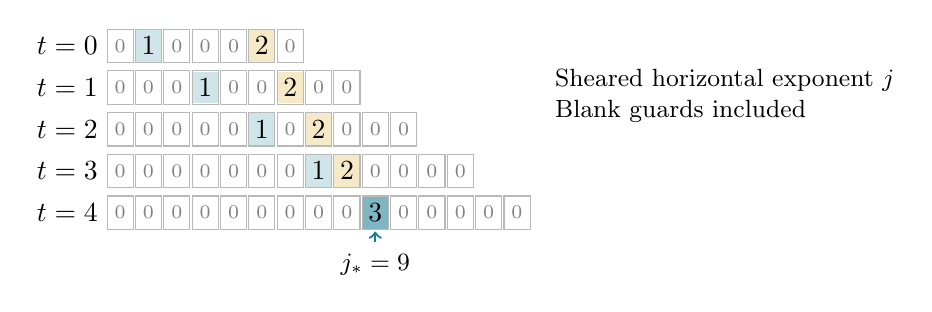
\begin{tikzpicture}[x=0.36cm,y=0.53cm]
 \foreach \t in {0,...,4} {
  \pgfmathtruncatemacro{\last}{6+2*\t}
  \node[anchor=east] at (-0.45,-\t) {$t=\t$};
  \foreach \j in {0,...,\last} {
   \draw[gray!55] (\j-0.46,-\t-0.40) rectangle (\j+0.46,-\t+0.40);
   \node[font=\scriptsize,text=gray] at (\j,-\t) {0};
  }
 }
 \foreach \t/\signal/\target in {0/1/5,1/3/6,2/5/7,3/7/8} {
  \fill[accent!20] (\signal-0.44,-\t-0.38) rectangle (\signal+0.44,-\t+0.38);
  \node at (\signal,-\t) {1};
  \fill[Goldenrod!25] (\target-0.44,-\t-0.38) rectangle (\target+0.44,-\t+0.38);
  \node at (\target,-\t) {2};
 }
 \fill[accent!55] (8.56,-4.38) rectangle (9.44,-3.62);
 \node at (9,-4) {3};
 \node[anchor=west,align=left,font=\small] at (15.0,-1.2)
    {Sheared horizontal exponent $j$\\Blank guards included};
 \draw[->,accent,thick] (9,-4.7)--(9,-4.45);
 \node[anchor=north,font=\small] at (9,-4.75) {$j_*=9$};
\end{tikzpicture}
\caption{The source-centre rows for $t<4$ and the terminal row at $t=4$.
The physical target remains at position $4$; its encoded position is
$4+t+1$, explaining the rightward shear.}
\label{fig:example}
\end{figure}

\subsection{All nonzero components}

The five auxiliary polynomials are
\begin{align*}
 D&=X^{14}Y^4,&
 Q&=X^6+X^8Y+X^{10}Y^2+X^{12}Y^3,\\
 B&=Y^4,&
 V&=1+Y+Y^2+Y^3,\\
 J&=Y^4\rep{9}.&&
\end{align*}
The final row is
\[
 T_3=X^9Y^4,\qquad
 T_0=Y^4\bigl(\rep{15}-X^9\bigr),\qquad T_1=T_2=0.
\]
The expression for $T_0$ is a polynomial with nonnegative coefficients:
subtraction here simply removes the accepting position from the full
zero--one row mask.

For compactness, the nonzero tile coefficients are listed by row as
positions carrying a given triple. Any tile not listed is zero.
\begin{center}
\small
\begin{tabular}{@{}cll@{}}
\toprule
Time & Triple & Horizontal positions\\
\midrule
$0$ & $001,010,100$ & $0;\ 1;\ 2$ respectively\\
    & $002,020,200$ & $4;\ 5;\ 6$ respectively\\
    & $000$ & $3$\\[2pt]
$1$ & $001,010,100$ & $2;\ 3;\ 4$ respectively\\
    & $002,020,200$ & $5;\ 6;\ 7$ respectively\\
    & $000$ & $0,1,8$\\[2pt]
$2$ & $001,010,102,020,200$ & $4;\ 5;\ 6;\ 7;\ 8$ respectively\\
    & $000$ & $0,1,2,3,9,10$\\[2pt]
$3$ & $001,012,120,200$ & $6;\ 7;\ 8;\ 9$ respectively\\
    & $000$ & $0,1,2,3,4,5,10,11,12$\\
\bottomrule
\end{tabular}
\end{center}
Each listed position $j$ on row $t$ contributes $X^jY^t$ to that triple's
polynomial. For example, the triple $120$ at $(j,t)=(8,3)$ outputs $3$;
its contribution is shifted by $XY$ to the accepting terminal monomial
$X^9Y^4$. The boundary coefficients are included in this list, not
suppressed as implicit blanks.

There are $73$ polynomial unknowns and $15$ reduced equations. The original
pair-colour form has $24$ equations, so the marginal projection removes
nine rows. The unique witness has $74$ nonzero coefficients across all
components and degree maxima
\[
 \deg_X^{\max}=14,\qquad \deg_Y^{\max}=4,\qquad \deg^{\max}=18.
\]
These agree with Proposition~\ref{prop:ledger}, including
$4^2+5\cdot4+5\cdot4+5+4+9=74$.

\subsection{The supplied expanded quadratic}

The file \codename{results/example\_system.json} gives every coefficient
of every reduced linear residual for this example. The complete
sum-of-squares polynomial has also been expanded exactly, not merely
specified by a proposed expansion procedure. In
\codename{results/example\_quadratic.json}, coefficients are polynomials
in $X,Y$, and monomials in the unknown names are recorded explicitly.
It contains $2{,}098$ nonzero monomials in the unknowns, or $5{,}082$
terms when their coordinate-polynomial coefficients are expanded as well.
Its degree in the unknowns is two, and its maximum coefficient total
degree in $X,Y$ is twelve. Exact evaluation at the supplied certificate
is zero.


\subsection{Feature-compressed versions of the same example}

For this four-symbol alphabet, choose either the two binary digits of a
symbol or the single integer-valued feature $\chi(a)=a$. The complete
counts are:
\begin{center}
\begin{tabular}{@{}lrrr@{}}
\toprule
Form & Unknowns & Equations & Maximum coefficient magnitude\\
\midrule
Pair colours & 73 & 24 & 1\\
Symbol marginals & 73 & 15 & 1\\
Binary features & 73 & 12 & 1\\
One weighted feature & 73 & 9 & 3\\
\bottomrule
\end{tabular}
\end{center}
All four systems accept the identical tuple described above, and their
\emph{entire} natural-polynomial zero sets coincide by the proved
reductions. The two feature systems and their fully expanded quadratics
are supplied in the corresponding \codename{example\_binary\_*} and
\codename{example\_weighted\_*} JSON files. Each feature quadratic has
$2{,}704$ nonzero unknown monomials and $12{,}364$ terms after expanding
coordinate coefficients. The coinciding term counts do not mean the two
polynomials are equal: their coefficients differ. Both are exactly
quadratic and vanish at the common certificate. Fewer linear rows have
increased the expanded polynomial size in this example, so the row savings
are not an arithmetic-operation optimum.

\section{Reproducibility and validation}
\label{sec:validation}

\subsection{Executable scope}

The package contains a dependency-free Python implementation using sparse
integer-coefficient dictionaries. It accepts any total finite deterministic
radius-one rule with quiescent blank, validates the alphabet and accepting
set, and emits the entire system, including both clocks and both
acceptance equations. It supports the reduced marginal form, the
unreduced pair-colour form, and arbitrary validated injective-feature maps. Polynomial equality is checked coefficientwise;
no floating-point arithmetic or numerical specialization is used.

The witness constructor takes a \emph{supplied external horizon} for the
purpose of generating or testing a candidate. The emitted mathematical
system contains no such horizon. The constructor deliberately returns a
candidate even when acceptance fails; the full residual check must then
reject it. This separation tests the acceptance conditions rather than
assuming them in the verifier.

Input rule tables are copied into immutable mappings. This prevents later
mutation of a caller's table from silently changing the meaning of an
already compiled system.

\subsection{Executed tests}

\begin{table}[ht]
\centering\small
\begin{tabular}{@{}p{0.49\linewidth}rr@{}}
\toprule
Test family & Candidates or cases & Result\\
\midrule
Ray-clock flows: coefficients $0,1,2$ on a $3\times3$ box,
three clock directions & $59{,}049$ & $11$ admitted\\
All $128$ quiescent binary rules, input lengths $1$--$4$,
horizons $0$--$4$ & $19{,}200$ & $1{,}280$ accepted\\
Seeded rules on $3$, $4$, and $5$ symbols, horizons $0$--$6$
& $840$ & $56$ accepted\\
Independent triple assignments on one-row tableaux
& $16{,}384$ & $32$ structurally valid\\
Pair/marginal structural zero-set comparisons on those assignments
& $16{,}384$ & All agree\\
Worked-certificate coefficient changes, off-region insertions,
and wrong horizons & $373$ & All rejected\\
Expanded quadratic: canonical and altered tuples & $8$ & Exact agreement\\
\bottomrule
\end{tabular}
\caption{Executed finite checks. ``Accepted'' means that the full residual
system vanishes exactly when the independently evaluated first-singleton
semantics holds. The pair/marginal line reuses the independent assignments,
so it is not an additional disjoint sample.}
\label{tab:tests}
\end{table}

The binary tests primarily stress the transition and boundary equations:
with accepting alphabet $\{1\}$, a binary input already containing a one
has an accepting event at time zero, while an all-zero input remains
blank. The multistate tests and the four-step worked example provide the
nontrivial later-acceptance cases. This limitation of the binary test set
is recorded rather than hidden behind its case count.

For the independent tile enumeration, each of three sites chooses any of
eight binary triples. Across sixteen specified rules and two one-letter
inputs, all $16\cdot2\cdot8^3=16{,}384$ assignments are checked. Exactly
one structural tableau per rule/input pair is admitted; its triples are
$(0,0,w_0)$, $(0,w_0,0)$, and $(w_0,0,0)$. The top row is formed from the
chosen outputs, and the actual linear equations must recover the valid
source and adjacency. These are not merely rechecks of the canonical
constructor's own tile choices.

The ray-clock enumeration allows coefficients equal to two, so it also
checks that nonnegative multiplicities are rejected rather than assuming
Boolean coefficients at input. The mutation tests delete or duplicate
every nonzero coefficient of the worked witness, insert coefficients
outside the region in every witness variable, and test six incorrect
horizons. Matrix-invariance tests compare different input lengths and
verify the stated coefficient sparsity and degree bounds.


The separate feature-verification run compares both binary and weighted
forms with the direct symbol system on $7{,}168$ binary
rule/input/horizon cases and $288$ seeded multistate cases. These are
$7{,}456$ cases with two feature-system checks per case, not an additional
claim of exhaustive validation of all polynomials. For each feature form,
all $367$ coefficient mutations of the worked tuple are rejected; two
exact expanded-quadratic evaluations agree with the linear residual
sum of squares. The run also checks the zero-feature singleton alphabet,
rejects three invalid feature maps, and verifies matrix invariance for
two feature forms. Its multistate seed is $20261003$; this is an arbitrary
integer seed, not a report date. The exact counts are recorded in
\codename{results/feature\_results.json}.

All these computations passed. They are finite validation, not a formal
proof of the infinite claims and not an independent proof-assistant audit.
The universal-machine reduction and the nondeterministic theorem rest on
the written proofs, not on an assertion that the finite examples establish
universality.

\subsection{Files and commands}

From the package root, with Python 3.10 or later, run
\begin{verbatim}
python code/verification.py
python code/export_quadratic.py
python code/feature_verification.py
pdflatex -interaction=nonstopmode -halt-on-error \
    unique_polynomial_histories.tex
pdflatex -interaction=nonstopmode -halt-on-error \
    unique_polynomial_histories.tex
\end{verbatim}
The Python commands rewrite the JSON results and the complete worked
example. The manuscript is a single self-contained TeX file with an
embedded bibliography and diagram; it does not depend on downloaded data
or on the repository being present locally. LaTeX requires the standard
packages listed in its preamble.

\section{Further research questions and concrete next steps}
\label{sec:research}

The following questions are proposed extensions of this construction.
They are not all asserted to be previously published open problems;
precise priority and existing special cases should be checked before a
separate novelty claim is made.

\subsection{A numerical universal matrix with a verified source table}

Choose a particular universal Turing-machine table with documented tape,
halt, and input conventions. Generate the cellular rule by
Proposition~\ref{prop:TM}, then emit its fixed matrix and input encoder.
A useful deliverable would contain the table, the simulation theorem,
all matrix entries, and a certificate checker, together with a numerical
value for $s^3+s+5$ and the chosen row count (in particular nine
in the weighted form). This would replace the generic universality
instantiation by a fully auditable concrete object. Minimizing $s$ is
secondary to obtaining a correct ordinary-input interface.

\subsection{Equation counts versus coefficient size}

The feature theorem gives an explicit tradeoff between the number of rows
and coefficient magnitude, without changing the witness tuple. Can the
nine-row weighted form be reduced further while retaining the fixed matrix,
canonical geometry, and full-tuple zero-set equivalence? For unit
coefficients, is there a substantially better alternative to
$6+3\lceil\log_2s\rceil$ rows? Any lower-bound problem must specify the
allowed fixed coordinate shifts and whether clock, geometry, and acceptance
constraints may be combined. The counting bound on feature-vector length
is not a lower bound for unrestricted linear systems. A finite-family
Pareto analysis should also count matrix density and expanded quadratic
size, which need not decrease with the number of rows.

\subsection{A one-coordinate compiler with the same uniqueness guarantees}

General linear-system undecidability over $\N[X]$ is known. The concrete
question here is whether one can retain a fixed matrix, a transparent
word-input map, Boolean-coefficient full witnesses, and first-history
single-foldness using only one coordinate indeterminate. A successful
construction must avoid the collisions of a fixed Kronecker substitution
and must prove uniqueness of any width or stride auxiliaries. This is a
sharpening target, not a proposed proof of a one-variable undecidability
threshold.

\subsection{Packing with an exact auxiliary-fibre ledger}

Can the canonical semiring witness be transferred to an ordinary integer
or exponential-Diophantine representation with a proved bijection, or at
least a controlled finite fibre, over the full auxiliary tuple? A useful
first milestone is a bounded version with explicit carry bounds and a
proof that every integer solution has a unique digit decomposition and
satisfies the polynomial coefficient equations. The unbounded extension
must confront Theorem~\ref{thm:nobound}; it cannot assume a computable
input-only degree limit.

\subsection{Parsimonious branching compilers}

Implement Theorem~\ref{thm:nondet} with labelled transition choices and
prove a root-counting correspondence for a carefully specified
nondeterministic machine semantics. Distinguish configuration histories,
labelled execution paths, and different schedules of independent actions.
These choices determine whether the target should count traces, events,
or equivalence classes. The existing equations already identify the point
at which local multiplicity becomes genuine computational branching.

\subsection{Smaller canonical regions}

The fixed expanding light cone is simple but can be much wider than the
actually visited tape interval. Can one use the minimal visited interval
while retaining unique nonnegative linear witnesses and a fixed matrix?
A naive freely chosen rectangle introduces padding ambiguity. Any
improvement needs a canonical extremum condition, with all witnesses
uniquely determined, rather than an existentially generous space bound.
A successful version could substantially reduce support size even when
it does not reduce the number of polynomial variables.

\subsection{Output-preserving and compositional interfaces}

The terminal polynomials already contain the whole final tape. A next
step is to specify a canonical output projection and prove that composing
two compilers preserves a bijection of complete witnesses. Input length,
head position, blank padding, and return-to-origin conventions must be
part of the interface. A composition theorem would make the normal form
useful as a library component rather than only as a universal acceptance
reduction.

\subsection{Kernel-checked support and reconstruction proofs}

A practical Lean or Rocq development should begin with finitely supported
maps $\N^2\to\N$, the coefficientwise ray-clock lemma, and the implication
``sum of natural coefficients equals one $\Rightarrow$ unique occupied
label.'' Next come the two shape identities, the missing blank marginal
row, and induction recovering the cellular evolution. Only after these
parts should one formalize the Turing-machine bridge and the exact count
ledger. The proof naturally separates algebraic identities, nonnegative
coefficient reasoning, finite-state semantics, and the universality input
reduction. No unbounded numerical search is required for these lemmas.

\section{Conclusion}

The central construction answers a precise design question: a deterministic
finite computation can have a fixed-arity, affine-linear certificate over
$\N[X,Y]$ in which the \emph{whole} witness, including clocks, boundaries,
and accepting-position marker, is unique. Nonnegative conservation forces
unit occupancy and a canonical light cone. Marginal matching then suffices
to reconstruct the local windows, and first acceptance removes arbitrary
post-acceptance extensions. Injective features compress the very same
witness relation to $6+3\lceil\log_2s\rceil$ unit-coefficient rows, or to
nine rows when symbol-sized coefficients are allowed. The reduction is
justified by already-forced one-hot occupancy, not by a generally false
claim that weighted marginals determine arbitrary multisets.

The resulting fixed-matrix problem is $\Sigma^0_1$-complete on
an unambiguous input family, even though every actual witness coefficient
is zero or one. The exact degree equals a linear function of the running
time, and no computable input-only bound on that degree is possible. A
single quadratic polynomial-semiring equation preserves all of these
properties; a bounded ordinary quadratic family preserves them only with
arity growing with the external bound.

The useful mathematical advance of this manuscript is the explicit
normal form and its witness-preserving reductions. Its limitations are
just as concrete: the unknowns are polynomials, the universal numerical
rule is not instantiated in the package, the main theorem is not yet
kernel-checked, and historical priority for the combined refinement
remains to be investigated. These boundaries leave a well-defined path
from the present proofs to a verified, compositional compiler and to
carefully audited ordinary-arithmetic packing experiments.

\clearpage
\appendix
\section{Notation and proof dependency ledger}

\begin{longtable}{@{}p{0.20\linewidth}p{0.73\linewidth}@{}}
\toprule
Symbol & Meaning\\
\midrule
\endhead
$\Sring$ & The semiring $\N[X,Y]$ of finite nonnegative-coefficient polynomials.\\
$X,Y$ & Fixed coordinate indeterminates, not numeric witness variables.\\
$\A,s,0$ & Cellular alphabet, its size, and its quiescent blank.\\
$f,\F$ & Radius-one local rule and accepting alphabet, with $0\notin\F$.\\
$w,m$ & Supplied finite input word and its length, $m\ge1$.\\
$h$ & Acceptance time recovered from a solution, not supplied to the system.\\
$w_t$ & Transition-row width $m+2t+2$.\\
$Z_{\ell c r}$ & Unknown polynomial indicating sites carrying a source triple.\\
$T_a$ & Unknown polynomial indicating terminal-row occurrences of symbol $a$.\\
$D,Q$ & Endpoint and prefix of the sheared right-boundary clock.\\
$B,V$ & Endpoint and prefix of the vertical clock.\\
$J$ & Unique horizontal prefix ending immediately before the accepting site.\\
$\LL_a,\CC_a,\RR_a,\OO_a$ & Linear forms for left, centre, right, and output symbols; not additional unknowns.\\
$I_a$ & Supplied input symbol-indicator polynomial.\\
$G$ & Linear form $V+B+Q+D$ for both blank source guards.\\
$H,K$ & Derived total tile and terminal polynomials; not additional unknowns.\\
$j_*$ & Encoded horizontal position of the unique accepting top cell.\\
\bottomrule
\end{longtable}

The proof order is
\[
 \text{ray clocks}
 \ \Longrightarrow\ \text{clock synchronization and shape}
 \ \Longrightarrow\ \text{unit occupancy},
\]
followed by
\[
 \text{marginal adjacency}
 \ \Longrightarrow\ \text{true windows}
 \ \Longrightarrow\ \text{true evolution}
 \ \Longrightarrow\ \text{first acceptance and uniqueness}.
\]
Boolean coefficient bounds are conclusions of this chain. They are never
used to justify the preceding shape equations. This ordering is part of
the soundness argument and should be preserved in any optimization or
formalization.

\section{Source and trust boundaries}

The repository review was tied to commit
\begin{center}
\small\texttt{e58b724c25bd34533b7a5834cfcbe873dfa01288}.
\end{center}
The root and Hilbert-tenth README files were inspected, together with
repository metadata and targeted searches. This is not a claim to have
audited every proof or every imported report in the repository.

The external literature establishes the pre-existing context and supplies
classical universality; it is not substituted for the displayed proofs of
shape, uniqueness, projection, or exact resource bounds. The code checks
finite instances and an explicit expanded polynomial. No Lean executable
was run, and no theorem in this manuscript is described as machine-checked
in a proof assistant.

The included code and results are original supporting artifacts for this
report. The reference papers are linked bibliographically, not bundled as
redistributed PDFs. Build intermediates and font files are not part of the
archive.

\begin{thebibliography}{9}

\bibitem{Narendran}
Paliath Narendran,
\emph{Solving linear equations over polynomial semirings},
in Proceedings of the 11th Annual IEEE Symposium on Logic in Computer
Science (LICS 1996), pp.~466--472, 1996.
\url{https://ieeexplore.ieee.org/document/561463/}.
The author's paper was also consulted through its accessible text mirror;
its polynomial power-forcing lemmas precede the present construction.

\bibitem{LohreySteinberg}
Markus Lohrey and Benjamin Steinberg,
\emph{Tilings and Submonoids of Metabelian Groups},
arXiv:0903.0648, 2009.
\url{https://arxiv.org/abs/0903.0648}.
In particular, see the subsemimodule construction and the zero-tiling-sum
problem.

\bibitem{Dong}
Ruiwen Dong,
\emph{Solving Homogeneous Linear Equations over Polynomial Semirings},
in 40th International Symposium on Theoretical Aspects of Computer Science
(STACS 2023), LIPIcs 254, article 26, pp.~26:1--26:19, 2023.
\url{https://doi.org/10.4230/LIPIcs.STACS.2023.26}.
Preprint: \url{https://arxiv.org/abs/2209.13347}.

\bibitem{Turing}
A.~M. Turing,
\emph{On Computable Numbers, with an Application to the
Entscheidungsproblem},
Proceedings of the London Mathematical Society, second series,
42 (1936--1937), pp.~230--265.
\url{https://doi.org/10.1112/plms/s2-42.1.230}.

\bibitem{ProveIt}
Vladimir Reshetnikov,
\emph{ProveIt}, repository snapshot
\texttt{e58b724c25bd34533b7a5834cfcbe873dfa01288},
inspected 2 October 2026.
Root overview and \texttt{Computability/HilbertTenthProblem/README.md}.
\url{https://github.com/VladimirReshetnikov/ProveIt/tree/e58b724c25bd34533b7a5834cfcbe873dfa01288}.

\end{thebibliography}
\end{document}
